\documentclass[a4paper]{article}

\usepackage[english]{babel}
\usepackage[utf8]{inputenc}
\usepackage{graphicx}
\usepackage{enumitem}
\usepackage{blindtext}

\graphicspath{ {./images/} }
\setlength\parindent{0pt}
    
\title{CS2500 Project 2 \\ 
       Run Time Complexity of Merge Sort, \\ 
       Quicksort, and Heapsort}
\author{Evan Wilcox}
\date{Due February 12, 2019}


\begin{document}
    \maketitle

    \section{Motivation}
    Knowing which sorting algorithm to choose when needing to sort something can be 
    difficult. Because certain algorithms work more efficiently on certain types
    of data sets being able to analyse these algorithms to find the best one 
    for a given situation can be very useful. \\

    This report will implement three algorithms in C++: merge sort, heap, sort and 
    quick sort. The algorithms will then be tested and analysed to find the inputs 
    that give the worst, best, and average runtimes for each algorithm.



    \section{Background}
    Each algorithm being analysed in this report uses a technique called recursion.
    Recursion is a method of solving a problem where you break the problem into smaller
    instances of the same problem. You can then solve the main problem by combining the 
    solutions of the smaller problems into the final solution. \\

    For example, merge sort starts by splitting the original array in half then calling
    merge sort on each half. Merge sort continually splits the array in half until
    the array only has one element. It then merges the smaller arrays back in
    to larger arrays until it is a sorted array. \\

    Similarly, quick sort splits the array into two subarrays. One that contains 
    elements that are less than some pivot element $p$. And one that contains elements 
    greater than $p$. It then puts the pivot element in between the two subarrays 
    then calls quicksort on each subarray resulting in a sorted array. \\

    Heap sort works a little differently. It starts by turning the array in to a max 
    heap. A max heap is a binary tree structure that keeps the heap sorted by keeping
    the highest element at the root of the tree and the smaller elements as leafs. 
    Heap sort then removes the max element and reheapifies the remaining array. What
    is left is a sorted array.





    \section{Procedures}
    \begin{enumerate}

        \item Develop a precondition, postcondition, and loop invariants for merge sort,
              quick sort, and heapsort.
        
        \item Show that the previous preconditions, postconditions, and loop invariants
              are correct.
        
        \item Express merge sort, quick sort, and heap sort using pseudocode.

        \item Implement merge sort, quick sort, and heap sort in python.
        
        \item Implement preconditions, postconditions, and invariants using python 
              assert statements to validate correctness.
        
        \item Measure run times of the three algorithms to experimentally determine 
              their run time complexity and compare to their expected run time 
              complexity.
        
        \item List problems encountered during development.
        
        \item Develop and implement a testing plan.

        \item Produce a conclusion addressing the efficacy of the methods used.
    \end{enumerate}

    
    \section{Pseudocode}
    \textbf{Heapsort Pseudocode} \\
    Max-Heapify$(A, i)$ \\ 
    1 $l=2i$ \\
    2 $r=2i+1$ \\
    3 \textbf{if} $l \leq A.heap$-$size$ and $A[l] > A[i]$ \\
    4 \phantom{hell}$largest = l$ \\
    5 \textbf{else} $largest = i$ \\
    6 \textbf{if} $4 \leq A.heap$-$size$ and $A[r] > A[largest]$ \\
    7 \phantom{hell}$largest = r$ \\
    8 \textbf{if} $largest \neq i$ \\
    9 \phantom{hell}exchange $A[i]$ with $A[largest]$ \\
    10 \phantom{he}Max-Heapify$(A, largest)$ \\

    Build-Max-Heap$(A)$ \\
    1 $A.heap$-$size = A.length$ \\
    2 \textbf{for} $i = \lfloor A.length/2 \rfloor$ \textbf{downto} 1 \\
    3 \phantom{hell}Max-Heapify$(A, i)$ \\

    Heap-Sort$(A)$ \\
    1 Build-Max-Heap$(A)$ \\
    2 \textbf{for} $i = A.length$ \textbf{downto} 2 \\
    3 \phantom{hell}exchange $A[1]$ with $A[i]$ \\
    4 \phantom{hell}$A.heap$-$size = A.heap$-$size - 1$ \\
    5 \phantom{hell}Max-Heapify$(A, 1)$ \\
    
    \newpage
    \textbf{Merge Sort Pseudocode} \\
    Merge$(A, p, q, r)$ \\
    1  $n_{1} = q-p+1$ \\
    2  $n_{2} = r-q$ \\
    3  let L$[1..n{1}+1]$ and $R[1..n_{2}+1]$ be new arrays \\
    4  \textbf{for} $i = 1$ to $n{1}$ \\
    5  \phantom{hell}$L[i] = A[p+i-1]$ \\
    6  \textbf{for} $j = 1$ \textbf{to} $n{2}$ \\
    7  \phantom{hell}$R[i] = A[q+j]$ \\
    8  $L[n_{1}+1] = \infty$ \\
    9  $R[n_{2}+1] = \infty$ \\
    10 $i = 1$ \\
    11 $j = 1$ \\
    12 \textbf{for} $k = p$ \textbf{to} $r$ \\
    13 \phantom{hell}\textbf{if} $L[i] \leq R[j]$ \\
    14 \phantom{hellhell}$A[k] = L[i]$ \\
    15 \phantom{hellhell}$i=i+1$ \\
    16 \phantom{hell}\textbf{else} $A[k] D R[j]$ \\
    17 \phantom{hellhell}$j=j+1$ \\

    Merge-Sort$(A, p, r)$ \\
    1 \textbf{if} $p<r$ \\
    2   \phantom{hell}$q = \lfloor (p + r)/2\rfloor $ \\
    3   \phantom{hell}Merge-Sort$(A, p, r)$ \\
    4   \phantom{hell}Merge-Sort$(A, p+1, r)$ \\
    5   \phantom{hell}Merge$(A, p, q, r)$ \\


    \vspace{1cm}
    \textbf{Quicksort Pseudocode} \\
    Quick-Sort$(A, p, r)$ \\
    1 \textbf{if} $p<r$ \\
    2 \phantom{hell}$q = $Partition$(A, p, r)$ \\
    3 \phantom{hell}Quick-Sort$(A, p, q-1)$ \\
    4 \phantom{hell}Quick-Sort$(A, q+1, r)$ \\

    Partition$(A, p, r)$ \\
    1 $x = A[r]$ \\
    2 $i = p - 1$ \\
    3 \textbf{for} $j = p$ to $r - 1$ \\
    4 \phantom{hell}\textbf{if} $A[j] \leq x$ \\
    5 \phantom{hellhell}$i = i + 1$ \\
    6 \phantom{hellhell}exchange $A[i]$ with $A[j]$ \\
    7 exchange $A[i + 1]$ with $A[r]$ \\
    8 \textbf{return} $i + 1$ \\



    \newpage
    \section{Problems Encountered}
    Originally the three algorithms were planned to be written, tested, and timed using
    Python but because of Python's overhead the expected results could not be achieved.
    Specifically, the QuickSort algorithm when implemented in Python ran out of memory, 
    hit the max recursion depth, or took an absurd amount of time even to sort small data
    sets. These problems were solved by implementing the three algorithms in C++ instead.

    \section{Testing Plan}
    All three algorithms were tested with the following testing plan: \\

    \begin{tabular}{ |l|l|l| }
        \hline
        \textbf{Input} & \textbf{Expected Output} & \textbf{Output Received} \\ \hline
        Empty Array & Empty Array & Empty Array \\ \hline
        $n < 0$ & Precondition Failed & Assert Error \\ \hline
        Unsorted Array, $n$ = length of array & Sorted Array & Sorted Array \\ \hline
        Sorted Increasing Array, $n$ = length of array & Sorted Array & Sorted Array \\ \hline
        Sorted Decreasing Array, $n$ = length of array & Sorted Array & Sorted Array \\ \hline
        Unsorted Array, $n <$ length of array & Sorted Array up to $n$ & Sorted Array up to $n$ \\ \hline
    \end{tabular}

    \section{Performance Results}
    The average case runtime for each algorithm is $n$lg$n$. This can be seen by 
    sorting an array of random integers. As shown in the graph below, all three 
    algorithms follow their expected average case runtime of $n$lg$n$. Heap sort 
    had the largest coefficient and quick sort had the smallest.\\
    \begin{center}
        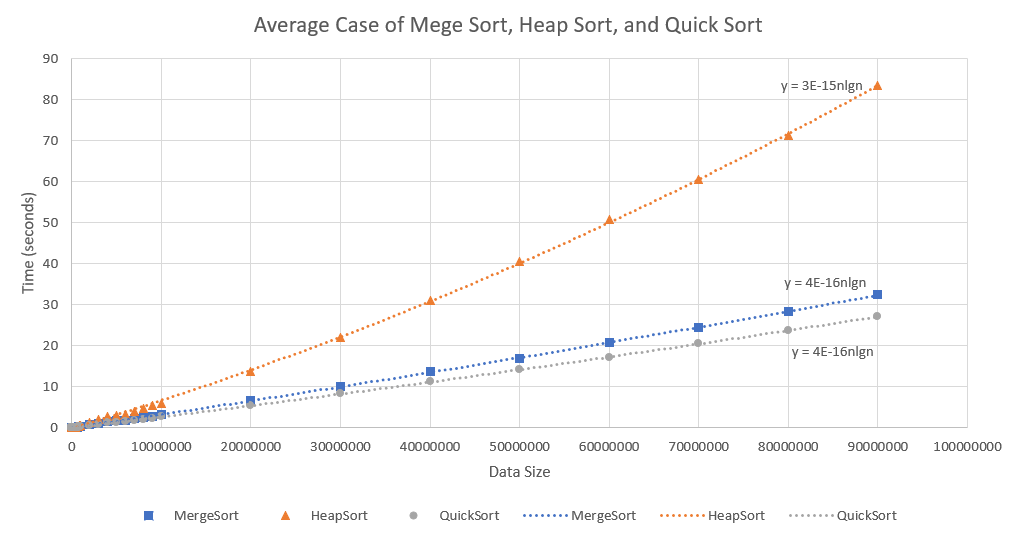
\includegraphics[scale=0.65]{Average}
    \end{center}

    \newpage
    The input that gives the best case runtime for each algorithm is different. For 
    merge sort it would be an array sorted in increasing order. This is because it
    would render the least amount of comparisons when merging. For heap sort it would
    be an array sorted in decreasing order because an array in decreasing order is 
    already a max heap so this reduces the amount of calls to heapify. For quick sort
    the input would be an array where every pivot element would split the array 
    exactly in half. Below is a graph comparing merge sort and heap sort's best
    case run time. Quick sort was not included because generating the input for quick
    sorts best case run time is significantly more difficult than merge sort and quick
    sort's.
    \begin{center}
        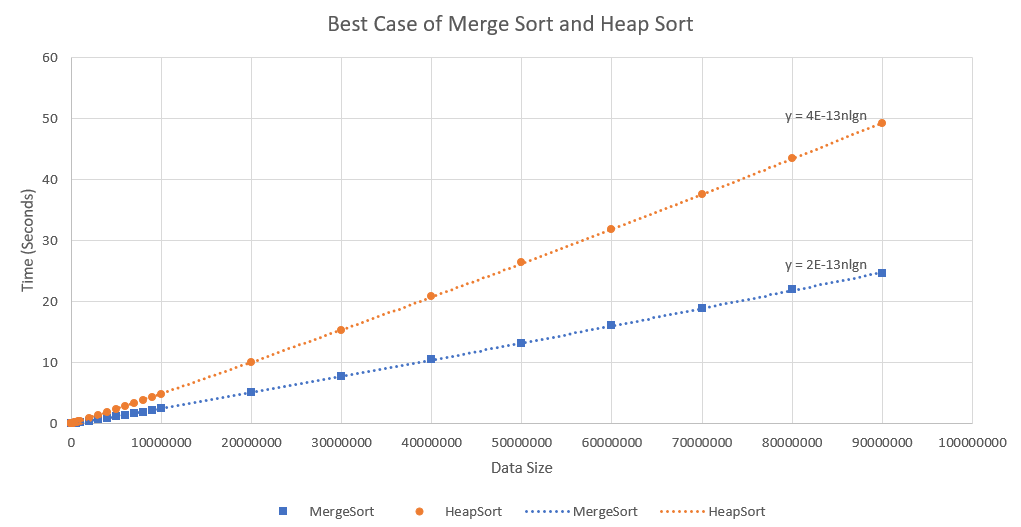
\includegraphics[scale=0.65]{Best}
    \end{center}
    
    Quick sort is the only one of the three algorithms whose expected worst case 
    runtime($n^{2}$) is different from its average case. The input that produces quick
    sort's worst case runtime would be an array whose pivot splits the array into a 
    zero length array and a $n-1$ length array, aka, the largest or smallest element in 
    the array. This array would look like a sorted array in increasing order. Both 
    merge sort and heap sort's worst case input would be an array that maximizes the
    amount of comparisons. These would look similar to arrays of random integers.
    \begin{center}
        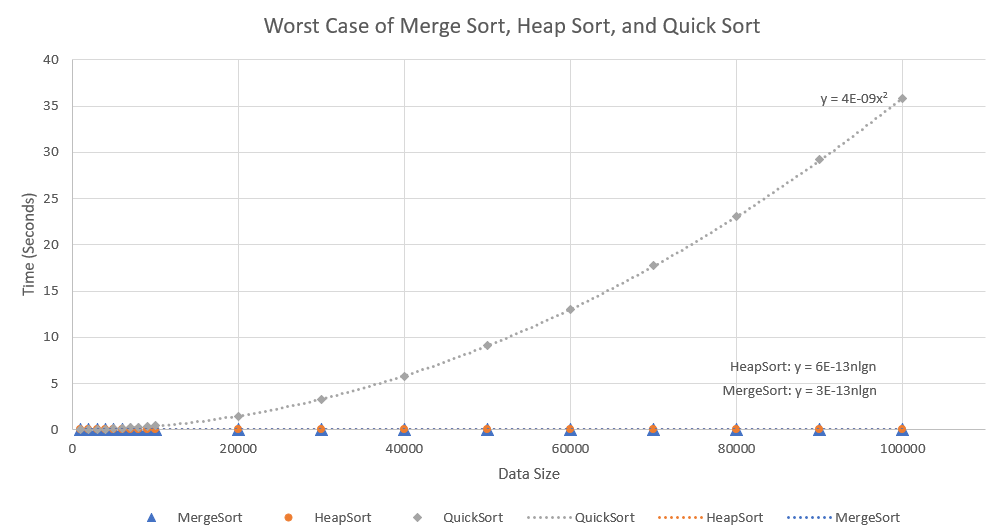
\includegraphics[scale=0.65]{Worst}
    \end{center}

    \section{Conclusion}
    In this report we showed that merge sort, heap sort, and quick sort meet their 
    expected runtime complexity for best, worst, and average case. We also showed the
    required inputs for each algorithm to produce their best, worst, and average case
    runtimes. Quick sort was found to have the lowest leading coefficient, which means
    it is more efficient. Except for the worst case where it has a runtime of $n^{2}$
    instead of $n$lg$n$. Heap sort was found to have the greatest leading coefficient
    which means it was the least efficient of the three algorithms.



    \newpage
    \textbf{Appendix A} - Source Code
    \begin{verbatim}
/////////////////////////////////////////
// @file   Sort.h
// @author Evan Wilcox
// @brief  Header file for Sort.cpp
/////////////////////////////////////////

#ifndef SORT_H
#define SORT_H
#include <iostream>
#include <assert.h>
using namespace std;

/////////////////////////////////////////
// @class Sort
// @brief Wrapper class for MergeSort, 
//        HeapSort, and QuickSort
/////////////////////////////////////////
class Sort
{
  private:
    bool debug;  // indictaes if debug mode is on

    /////////////////////////////////////////
    // @fn     swap
    // @brief  swaps the values at *a and *b
    // @pre    a and b are pointers
    // @post   the values of a* and b* are swapped
    // @param  a pointer to an int
    // @param  b pointer to an int
    // @return none
    /////////////////////////////////////////
    void swap(int *a, int *b);

    /////////////////////////////////////////
    // @fn     checkSort
    // @brief  checks if the passed array is in increasing order
    // @pre    0 <= l <= r
    // @post   true is returned if the subarry arr[l..r] is in increasing order
    // @param  arr the array containing the subarry to be checked
    // @param  l is the first index of the array to be checked
    // @param  r is the last index of the array to be cecked
    // @return bool b is true if the array is in increasing order
    /////////////////////////////////////////
    bool checkSort(int arr[], int l, int r);

    /////////////////////////////////////////
    // @fn     checkHeap
    // @brief  checks if the node i is a max heap
    // @pre    heapSize and i >= 0
    // @post   true is returned if the node i is a max heap
    // @param  arr the array containing the the node i
    // @param  heapSize the size of the heap in the the array arr
    // @praam  i the node that is being checked
    // @return returns true if the node i is a max heap
    /////////////////////////////////////////
    bool checkHeap(int arr[], int heapSize, int i);

    /////////////////////////////////////////
    // @fn     merge
    // @brief  merges two sorted subarrays
    // @pre    the subarrays arr[l..m] and arr[m+1..r] are in increasing order
    //         0 <= l <= m <= r
    // @post   the two subarrays are merged
    // @param  arr the array containing the subarrays to be sorted
    // @param  l left index of the first array
    // @param  m the middle index between the two subarrays
    // @param  r right index of the second subarray
    // @return none
    /////////////////////////////////////////
    void merge(int arr[], int l, int m, int r);

    /////////////////////////////////////////
    // @fn     heapify
    // @brief  turns the node i into a max heap
    // @pre    n and i >= 0
    // @post   the node i is a max heap
    // @param  arr the array containing the node i 
    // @param  n the heapsize of the heap in the array arr
    // @param  i the node to be turned into a max heap
    // @return none
    /////////////////////////////////////////
    void heapify(int arr[], int n, int i);

    /////////////////////////////////////////
    // @fn     partition
    // @brief  partitions the subarry arr[l..h]
    // @pre    0 <= l <= h
    // @post   the subarray arr[l..h] is partitioned
    // @param  arr the array containing the subarry to be pratitioned
    // @param  l the left index of the subarry
    // @param  h the right index of the subarray
    // @return the index of the element used as the partition
    /////////////////////////////////////////
    int partition(int arr[], int l, int h);

  public:
    /////////////////////////////////////////
    // @fn     Sort
    // @brief  default constructor
    // @pre    none
    // @post   Sort object is created
    // @return none
    /////////////////////////////////////////
    Sort();

    /////////////////////////////////////////
    // @fn     Sort
    // @brief  constructor that sets debug
    // @pre    none
    // @post   Sort object is created
    // @param  b the debug mode to be set
    // @return none
    /////////////////////////////////////////
    Sort(bool b);

    /////////////////////////////////////////
    // @fn     setDebug
    // @brief  changes the debug mode
    // @pre    none
    // @post   debug = b
    // @param  b the new debug mode
    // @return none
    /////////////////////////////////////////
    void setDebug(bool b); 

    /////////////////////////////////////////
    // @fn     print
    // @brief  prints out the given array
    // @pre    n >= 0
    // @post   arr is printed out using cout
    // @param  arr and array of integers
    // @param  n the length of arr
    // @return none
    /////////////////////////////////////////
    void print(int arr[], int n);

    /////////////////////////////////////////
    // @fn     mergeSort
    // @brief  recursive implementation of the quicksort algorithm
    // @pre    0 <= l <= r
    // @post   arr[l..r] is sorted in increasing order
    // @param  arr the array containing the subarry to be sorted
    // @param  l the left index of the subarry
    // @param  r the right index of the subarray
    // @return none
    /////////////////////////////////////////
    void mergeSort(int arr[], int l, int r);

    /////////////////////////////////////////
    // @fn     heapSort
    // @brief  recursive implementation of heapsort
    // @pre    n is the length of arr,
    //         0 <= n
    // @post   arr is in increasing order
    // @param  arr the array to be sorted
    // @param  n the length of arr
    // @return none
    /////////////////////////////////////////
    void heapSort(int arr[], int n);

    /////////////////////////////////////////
    // @fn     quickSort
    // @brief  recursive implementation of quicksort
    // @pre    0 <= l <= h
    // @post   arr[l..h] is in increasing order
    // @param  arr the array containing the subarry to be sorted
    // @param  l the left index of the subarry to be sorted
    // @param  h the right index of the subarry to be sorted
    // @return none
    /////////////////////////////////////////
    void quickSort(int arr[], int l, int h);
};

#endif


////////////////////////////////////////////////////
// @file   Sort.cpp
// @author Evan Wilcox
// @brief  Function definitions for the Sort class
////////////////////////////////////////////////////

#include "Sort.h"

void Sort::swap(int *a, int *b)
{
  int temp = *a;
  *a = *b;
  *b = temp;
}


bool Sort::checkSort(int arr[], int l, int r)
{
  // Precondition
  if(debug)
  {
    assert(0 <= l);
    assert(l <= r);
  }
  
  for(int i = l; i < r-1; i++)
  {
    if(arr[i] > arr[i+1])
    {
      return false;
    }
  }

  return true;
}


bool Sort::checkHeap(int arr[], int heapSize, int i)
{
  // Precondition
  if(debug)
  {
    assert(0 <= heapSize);
    assert(0 <= i);
  }
  
  if((i * 2 + 1) < heapSize)
  {
    if(arr[i*2+1] > arr[i])
    {
      return false;
    }
  }

  if((i * 2 + 2) < heapSize)
  {
    if(arr[i*2+2] > arr[i])
    {
      return false;
    }
  }

  return true;
}


void Sort::merge(int arr[], int l, int m, int r)
{
  // Preconditions
  if(debug)
  {
    assert(0 <= l);
    assert(l <= m);
    assert(m <= r);
    assert(checkSort(arr, l, m));
    assert(checkSort(arr, m+1, r));
  }


  int i, j, k;
  int n1 = m - l + 1;
  int n2 = r - m;

  int *L = new int[n1];
  int *R = new int[n2];

  for(i = 0; i < n1; i++)
  {
    L[i] = arr[l+i];
  }
  for(j = 0; j < n2; j++)
  {
    R[j] = arr[m+1+j];
  }

  i = 0;
  j = 0;
  k = l;
  
  ////////////////////////////////////////////
  // merges the arrays L and R in to arr 
  // loop precondition:  arrays L and R are in sorted increasing order
  // loop postconsition: arr[l..r] is in increasing order
  // ivariant: arr[l..k] contains the smalest elements from 
  //           L and R in increasing order
  // proof:
  //    initialization: before the loop k=l so the subarry arr[l..k] 
  //                    has no elements so it is sorted
  //
  //    maintenance: either an element from L or R gets moved to arr
  //                 and k increases each iteration so arr[l..k] still 
  //                 contains elements from L and R
  //
  //    termination: at termination k = r so the subarry arr[l..r] contains 
  //                 the smallest elements from L and R at termination
  //
  ///////////////////////////////////////////
  while(i < n1 && j < n2)
  {
    // Invariant
    if(debug)
    {
      assert(checkSort(arr, l, k));
    }
    
    if(L[i] <= R[j])
    {
      arr[k] = L[i];
      i++;
    }
    else
    {
      arr[k] = R[j];
      j++;
    }
    k++;
  }

  while(i < n1)
  {
    arr[k] = L[i];
    i++;
    k++;
  }

  while(j < n2)
  {
    arr[k] = R[j];
    j++;
    k++;
  }

  delete L;
  delete R;

  // Postcondiion
  if(debug)
  {
    assert(checkSort(arr, l, r));
  }
}


void Sort::heapify(int arr[], int n, int i)
{
  // Preconditions
  if(debug)
  {
    assert(n >= 0);
    assert(i >= 0);
  }
  
  int largest = i;
  int l = 2*i + 1;
  int r = 2*i + 2;

  if(l < n && arr[l] > arr[largest])
  {
    largest = l;
  }

  if(r < n && arr[r] > arr[largest])
  {
    largest = r;
  }

  if(largest != i)
  {
    swap(&arr[i], &arr[largest]);
    heapify(arr, n, largest);
  }

  // Postcondition
  if(debug)
  {
    assert(checkHeap(arr, n, largest));
  }
}


int Sort::partition(int arr[], int l, int h)
{
  // Precondition
  if(debug)
  {
    assert(0 <= l);
    assert(l <= h);
  }
  
  int x = arr[h];
  int i = (l - 1);

  for(int j = l; j <= h-1; j++)
  {
    if(arr[j] <= x)
    {
      i++;
      swap(&arr[i], &arr[j]);
    }
  }

  swap(&arr[i+1], &arr[h]);
  return (i+1);
}


Sort::Sort()
{
  debug = false;
}


Sort::Sort(bool b)
{
  debug = b;
}


void Sort::setDebug(bool b)
{
  debug = b;
}


void Sort::print(int arr[], int n)
{
  // Precondition
  if(debug)
  {
    assert(0 <= n);
  }
  
  for(int i = 0; i < n-1; i++)
  {
    cout << arr[i] << ", ";
    if((i+1) % 10 == 0)
    {
      cout << endl;
    }
  }

  cout << arr[n-1] << endl << endl;
}


void Sort::mergeSort(int arr[], int l, int r)
{
  // Preconditions
  if(debug)
  {
    assert(0 <= l);
    assert(l <= r);
  }
  
  if(l < r)
  {
    int m = l+(r-l)/2;

    mergeSort(arr, l, m);
    mergeSort(arr, m+1, r);
    merge(arr, l, m, r);
  }

  // Postcondition
  if(debug)
  {
    assert(checkSort(arr, l, r));
  }
}


void Sort::heapSort(int arr[], int n)
{
  // Preconditions
  if(debug)
  {
    assert(0 <= n);
  }
  
  ////////////////////////////////////////////
  // this for loop builds a max heap
  // loop precondition:  n is the number of elements in arr
  // loop postconsition: arr is not a max heap
  // ivariant: the nodes i+1, i+2, .., n are roots of 
  //           a max heap
  // proof:
  //    initialization: i = n/2 so the nodes n/2 +1, n/2 +2,
  //                    ..., n are leafs so are trivial roots of
  //                    max heaps
  //
  //    maintenance: the children of i are numbered higher than i,
  //                 by the loop invariant they are both roots of max heaps
  //                 decrementing i restablishes the invariant
  //
  //    termination: at termination i = -1, each node 1, 2, 3 are 
  //                 roots of max heaps
  //
  ///////////////////////////////////////////
  for(int i = n/2 - 1;i >= 0; i--)
  {
    heapify(arr, n, i);

    // Invariant
    if(debug)
    {
      for(int j = n/2; j < n; j++)
      {
        assert(checkHeap(arr, n, j));
      }
    }
  }
  
  for(int i = n-1; i >= 0; i--)
  {
    swap(&arr[0], &arr[i]);
    heapify(arr, i, 0);
  }

  // Postcondition
  if(debug)
  {
    assert(checkSort(arr, 0, n));
  }
}


void Sort::quickSort(int arr[], int l, int h)
{
  // Preconditions
  if(debug)
  {
    assert(0 <= l);
    assert(l <= h);
  }
  
  if(l < h)
  {
    int p = partition(arr, l, h);
    quickSort(arr, l, p-1);
    quickSort(arr, p+1, h);
  }

  // Postcondition
  if(debug)
  {
    assert(checkSort(arr, l, h));
  }
}




///////////////////////////////////////////////
// @file   main.cpp
// @author Evan Wilcox
// @brief  Program used to test the Sort Class
///////////////////////////////////////////////

#include <iostream>
#include "Sort.h"
#include <random>
#include <time.h>
using namespace std;

int main()
{  
  Sort S;
  S.setDebug(true);

  const unsigned long MAX_SIZE = 1000000000;

  int *A = new int[MAX_SIZE];
  int *B = new int[MAX_SIZE];
  int *C = new int[MAX_SIZE];

  int rInt;
  clock_t t;

  unsigned n = 10;
  unsigned k = n;
  
  // Testing the algorithms with arrays of random integers to find average runtime.
  for( ; n < 10000; n+=k)
  {
    cout << "n = " << n << endl;

    for(unsigned j = 0; j < n; j++)
    {
      rInt = rand() % (n*10);
      A[j] = rInt;
      B[j] = rInt;
      C[j] = rInt;
    }

    t = clock();
    S.mergeSort(A, 0, n-1);
    cout << "MergeSort: " << (float)(clock()-t)/CLOCKS_PER_SEC << endl;

    t = clock();
    S.heapSort(B, n);
    cout << "HeapSort:  " << (float)(clock()-t)/CLOCKS_PER_SEC << endl;

    t = clock();
    S.quickSort(C, 0, n-1);
    cout << "QuickSort: " << (float)(clock()-t)/CLOCKS_PER_SEC << endl << endl;

    if(n == k*10)
    {
      k = n;
    }
  }
  

  n = 10;
  k = n;
  // Testing the algorithms with sorted arrays to find best/worst runtime.
  for( ; n < MAX_SIZE; n+=k)
  {
    cout << "n = " << n << endl;

    for(unsigned j = 0; j < n; j++)
    {
      A[j] = j;
      B[j] = n-j;
      C[j] = j;
    }

    t = clock();
    S.mergeSort(A, 0, n-1);
    cout << "MergeSort: " << (float)(clock()-t)/CLOCKS_PER_SEC << endl;

    t = clock();
    S.heapSort(B, n);
    cout << "HeapSort:  " << (float)(clock()-t)/CLOCKS_PER_SEC << endl;

    t = clock();
    S.quickSort(C, 0, n-1);
    cout << "QuickSort: " << (float)(clock()-t)/CLOCKS_PER_SEC << endl << endl;

    if(n == k*10)
    {
      k = n;
    }
  }

  delete A;
  delete B;
  delete C;

  return 0;
}
    \end{verbatim}

\end{document}